\documentclass[12pt]{article}
\usepackage{amsmath}
\usepackage{amssymb}
\usepackage{amsthm}
\usepackage{geometry}
\usepackage{graphicx}
\usepackage{subcaption}
\usepackage{enumitem}
\usepackage{listings}
\usepackage{ulem}
\usepackage[table]{xcolor}
\usepackage{tikz-cd}
\usepackage{tcolorbox}
\usepackage{array}
\usepackage{mdframed}
\usepackage{cancel}
\usepackage{hyperref}

% Set the top margin

\geometry{top=1in} % You can adjust the measurement as needed


\begin{document}
\begin{titlepage}
\centering
\vspace*{\fill} % Adds vertical space to center the title block vertically
{\Huge Topology} \\[0.5cm] % Title 2
{\Huge Home Work 5}\\[1.5cm] % Title 3
{\Large Student: 26-712-224}\\[0.5cm] % Student ID
{\Large \today} % Date, \today adds today's date
\vspace*{\fill}
\end{titlepage}

\newpage
\noindent
\noindent\textbf{Exercise 1.}
Let $\mathbb{S}^1$ denote the unit circle (equipped with the topology induced from $\mathbb{R}^2$), let $\mathbb{R}_\infty = \mathbb{R} \cup \{\infty\}$ and let $P : \mathbb{S}^1 \to \mathbb{R}_\infty$ be the map defined by
\begin{align*}
P(x,y) =
\begin{cases}
\dfrac{2x}{1-y}, & \text{if } (x,y) \neq (0,1),\\
\infty, & \text{if } (x,y) = (0,1).
\end{cases}
\end{align*}
\begin{center}
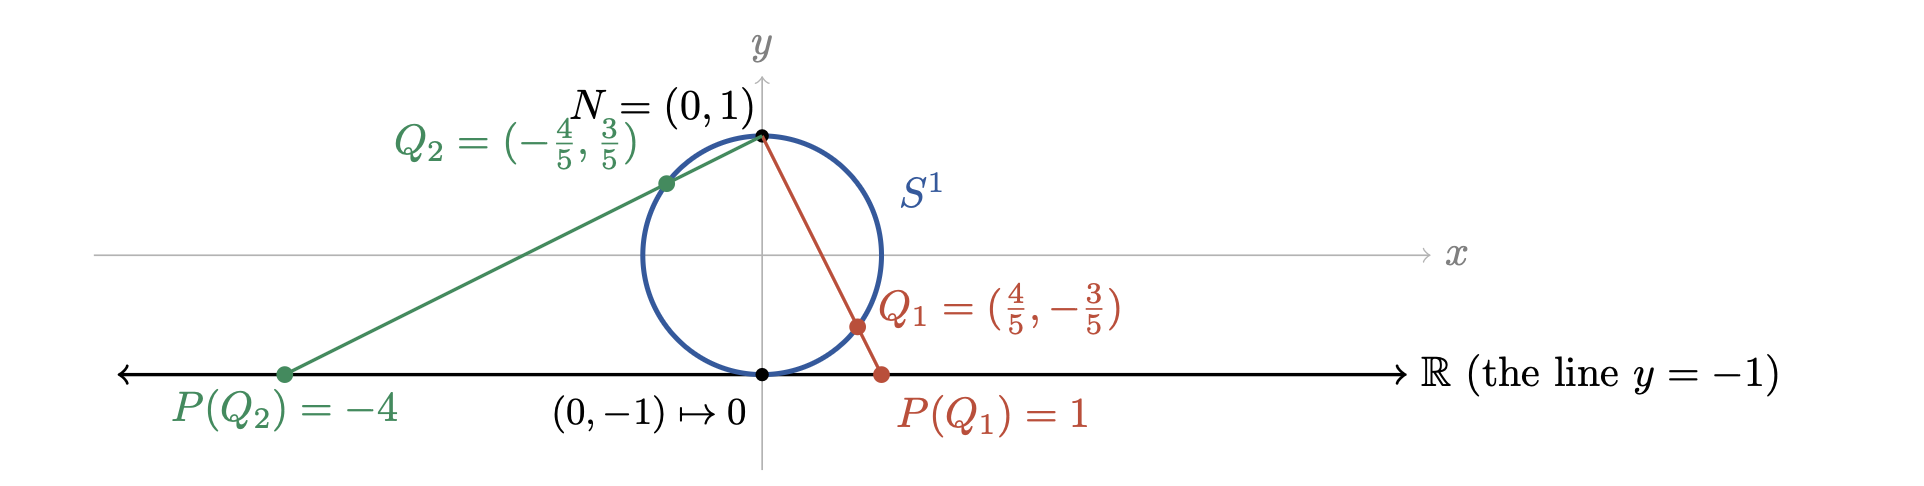
\includegraphics[width=0.85\linewidth]{Diagrams/Topology_WK_6_Q1.png}
\end{center}
This map is known as stereographic projection. Let $\mathcal{U}_{\mathbb{R}_\infty}$ denote the quotient topology on $\mathbb{R}_\infty$ induced by $P$.
\begin{enumerate}
\item[(i)] Prove that for all $a < b \in \mathbb{R}$, $(a,b) \in \mathcal{U}_{\mathbb{R}_\infty}$.
\item[(ii)] Let $\mathcal{B}_\infty = \{(-\infty,a) \cup (b,+\infty) \cup \{\infty\} : a < b \in \mathbb{R}\}$, and prove that $\mathcal{B}_\infty$ forms a base of open neighborhoods of the point $\infty$.
\item[(iii)] Prove that $\{(a,b) : a,b \in \mathbb{R}\} \cup \mathcal{B}_\infty$ form a basis for $\mathcal{U}_{\mathbb{R}_\infty}$. (You can use the face that arcs on $\mathbb{S}^1$ form a base for its topology.)
\end{enumerate}

\clearpage

\noindent\textbf{Exercise 2.}
The goal of this exercise is to prove that the Hausdorff property is not preserved by quotients. Consider two lines on the plane $L_0 = \{(x,0); x \in \mathbb{R}\}$, $L_1 = \{(x,1); x \in \mathbb{R}\}$, and equip $L = L_0 \cup L_1$ with the topology induced by $\mathbb{R}^2$. Now consider the equivalence relation on $L$ defined as
\begin{align*}
(x,0) \sim (y,1) \quad \text{iff } x = y < 0
\end{align*}
and define the space $X = L/{\sim}$ (with quotient topology), along with the projection $p : L \to X$.
\begin{enumerate}
\item[i)] Show that $L$ is Hausdorff.
\item[ii)] Let $x_1 < 0 < x_2$ and define $P_1 = p(x_1,0) = p(x_1,1)$, $P_2^+ = p(x_2,1)$, $P_2^- = p(x_2,0)$, $P_0^+ = p(0,1)$, $P_0^- = p(0,0)$. Describe the neighbourhoods in $X$ of $P_1$, $P_0^+$, $P_0^-$, $P_2^+$ and $P_2^-$.
\item[iii)] Prove that $X$ is \emph{not} Hausdorff.
\end{enumerate}
\begin{center}
\begin{tikzpicture}[scale=1.1]
\draw (-3,0) -- (0,0);
\draw (0,1) -- (3.5,1);
\draw (0,-1) -- (3.5,-1);
\draw[dotted] (0,-1) -- (0,1);
\draw[fill=white] (0,0) circle (2pt);
\fill (-2,0) circle (2pt) node[above] {$P_1$};
\fill (0,1) circle (2pt) node[above] {$P_0^+$};
\fill (0,-1) circle (2pt) node[below] {$P_0^-$};
\fill (2,1) circle (2pt) node[above] {$P_2^+$};
\fill (2,-1) circle (2pt) node[below] {$P_2^-$};
\end{tikzpicture}
\end{center}

\clearpage

\noindent\textbf{Exercise 3.}
The goal of this exercise is to show that two definitions of the torus are topologically equivalent, namely that
\begin{align*}
\mathbb{R}^2/\mathbb{Z}^2 \cong \mathbb{S}^1 \times \mathbb{S}^1.
\end{align*}
Consider $\mathbb{R}^2/\mathbb{Z}^2$ with the quotient topology arising from the natural group action of $\mathbb{Z}^2$ on $\mathbb{R}^2$: for $(n,m) \in \mathbb{Z}^2$, $(x,y) \in \mathbb{R}^2$, we define $(n,m)\cdot(x,y) = (n+x,m+y)$. Let $p : \mathbb{R}^2 \to \mathbb{R}^2/\mathbb{Z}^2$ be the quotient map. The topology on $\mathbb{S}^1$ is just the induced topology by considering $\mathbb{S}^1$ as the circle of unit radius in $\mathbb{R}^2$, and the topology on $\mathbb{S}^1 \times \mathbb{S}^1$ is the product topology.
\begin{enumerate}
\setlength{\itemsep}{2pt}
\item[(i)] Let $\psi : \mathbb{R}^2 \to \mathbb{S}^1 \times \mathbb{S}^1$ be the map defined by
\begin{align*}
\psi(x,y) = \left(e^{2\pi ix},e^{2\pi iy}\right).
\end{align*}
Show that $\psi$ descends to a well-defined map $\bar{\psi} : \mathbb{R}^2/\mathbb{Z}^2 \to \mathbb{S}^1 \times \mathbb{S}^1$, such that $\psi = \bar{\psi} \circ p$. Show that $\bar{\psi}$ is a bijection.
\begin{center}
\begin{tikzcd}[row sep=small,column sep=large]
\mathbb{R}^2 \arrow[d,"p"'] \arrow[dr,"\psi"] & \\
\mathbb{R}^2/\mathbb{Z}^2 \arrow[r,"\bar{\psi}"'] &
\mathbb{S}^1 \times \mathbb{S}^1
\end{tikzcd}
\end{center}
\item[(ii)] Use the definition of the quotient topology to check that $p$ is continuous.
\item[(iii)] Prove that $p$ is an open map. (For the definition of an open map, see Exercise 3 of Problem Sheet 4.)

[Hint: For $U \subset \mathbb{R}^2$, show that
\begin{align*}
p^{-1}(p(U)) = \bigcup_{a \in \mathbb{Z}^2}(a+U).
\end{align*}
Here the notation is $a+U := \{a+x : x \in U\}$ - this is a translation of the set $U$ by $a$.]
\item[(iv)] Use the definition of product topology to show that $\psi$ is continuous. (You can use Exercise 3 of Problem Sheet 4.)
\item[(v)] Prove that $\psi$ is an open map.

[Hint: Start with a base consisting of rectangles for the topology on $\mathbb{R}^2$.]
\item[(vi)] Deduce that $\bar{\psi}$ is both continuous and open, and hence a homeomorphism.

[Hint: Use that for $U \subset \mathbb{R}^2/\mathbb{Z}^2$, $p(p^{-1}(U)) = U$, and hence
\begin{align*}
\bar{\psi}(U)
= \bar{\psi}\left(p\left(p^{-1}(U)\right)\right)
= \psi\left(p^{-1}(U)\right).
\end{align*}
Find a similar formula for $\bar{\psi}^{-1}(V)$ where $V \subset \mathbb{S}^1 \times \mathbb{S}^1$.]
\end{enumerate}

\clearpage

\noindent\textbf{Exercise 4.}
Recall that the real projective space $\mathbb{RP}^n$ is defined as the set of lines going through the origin:
\begin{align*}
\mathbb{RP}^n = \{L_x : x \in \mathbb{R}^{n+1} \setminus \{0\}\},
\end{align*}
where $L_x$ is the line passing through $0 \in \mathbb{R}^{n+1}$ and $x$, we can equip $\mathbb{RP}^n$ with the quotient topology $\mathcal{U}_p$, induced by the surjective map $p : \mathbb{R}^{n+1} \setminus \{0\} \to \mathbb{RP}^n$:
\begin{align*}
x \mapsto L_x.
\end{align*}
Our goal is to show that $\mathbb{RP}^n$ is homeomorphic to $\mathbb{S}^n/\{\pm 1\}$.
\begin{enumerate}
\item[(i)] For every set $U \subset \mathbb{R}^{n+1}$, show that for every $y \in p(U)$, there exists $x \in U$, such that $L_y = L_x$.
\item[(ii)] Show that
\begin{align*}
p^{-1}(p(U)) = \bigcup_{\lambda \in \mathbb{R}^*}(\lambda U),
\end{align*}
where $\lambda U = \{\lambda x : x \in U\}$ - this is the homothethy set of $U$ by ratio $\lambda$).
\item[(iii)] Conclude that $p$ is an open map.
\item[(iv)] By following a similar strategy as in Exercise 3, show that $\mathbb{RP}^n$ is homeomorphic to $\mathbb{S}^n/\{\pm 1\}$ via the following diagram.
\begin{center}
\begin{tikzcd}[row sep=large,column sep=large]
\mathbb{R}^{n+1}\setminus\{0\}
    \arrow[r,"p'"] \arrow[d,"p"'] &
\mathbb{S}^n \arrow[d,"\psi"] \\
\mathbb{RP}^n \arrow[r,"\bar{\psi}"'] &
\mathbb{S}^n/\{\pm 1\}
\end{tikzcd}
\end{center}
\end{enumerate}

\clearpage

\noindent\textbf{Exercise 5.}
Equip the set $\{0,1\}$ with the discrete topology, let $X = \{0,1\}^{\mathbb{N}}$, and consider the sequence $(e_n)_{n=1}^{\infty}$ in $X$ where $e_i$ has a $1$ in position $i$ and $0$s everywhere else.
\begin{enumerate}
\item[(i)] Equip $X$ with the box topology $\mathcal{U}_{\mathrm{Box}}$, and prove that the sequence $(e_n)_{n=1}^{\infty}$ does not have a convergent subsequence.
\item[(ii)] Show that $(e_n)$ converges in product topology.
\end{enumerate}

\clearpage

\noindent\textbf{Exercise 6. (Universal property for quotient topology.)}
Let $(X,\mathcal{U})$ be a topological space, and $Y$ a set with a surjective map $p : X \to Y$. Prove that the quotient topology $\mathcal{U}_Y$ on $Y$ is the unique topology of $Y$ such that, for every topological space $(Z,\mathcal{V})$ and map $f : Y \to Z$, $f$ is continuous if and only if $f \circ p : X \to Z$ is continuous.
\begin{center}
\begin{tikzcd}[row sep=large,column sep=large]
& (X,\mathcal{U})
    \arrow[d,"p"]
    \arrow[dl,dashed,"f\circ p"'] \\
(Z,\mathcal{V}) & (Y,\mathcal{U}_Y) \arrow[l,"f"]
\end{tikzcd}
\end{center}


\end{document}
